\documentclass[20pt]{letter}
\usepackage{amsmath}
\usepackage{amsthm}
\usepackage{amssymb}
\usepackage{fullpage}
\usepackage{graphicx}
\usepackage{geometry}
 \geometry{
 a4paper,
 total={180mm,257mm},
 left=12mm,
 top=20mm,
 }

\newcommand{\abs}[1]{{\left\lvert #1 \right\rvert}}	
\newenvironment{solution}{\textbf{Solution:}}{\hfill$\square$}


\begin{document}

\begin{center}
{\LARGE \textbf{
CS685 - Data Mining\\
2020-2021-I: Assignment 2
}}\end{center}

{\Large
Name: Sarthak Singhal        ~~~~~~~~~~~~~~~~~~~~~~~~~~~~~~~~~~~~~~~~~~~~~~~~~~~~~~~~~~   Roll No.: 170635\\\\}
%If you discuss the question with someone, please mention their name on your assignment. Remember, you are allowed to discuss and not copy.
%You can use any theorem used in the class except if that theorem itself needs to be proven in the question.

%Please print on both sides while submitting the assignment.


% Based on decoding of Reed Solomon codes

\begin{enumerate}
{ \Large
\item \textbf{Question 13}
}
{ \fontsize{13}{18}\selectfont\\\\
%Write your solution here.
\textbf{Assumptions made in the assignment:}
\begin{itemize}
    \item Undirected graph is used for finding connected components in Question 5.
    \item In questions 6,7,10,11, I have ignored the paths where src $\rightarrow$ dest is not reachable and where src == dest.
    \item In questions 8,9, I have only ignored the paths where src $\rightarrow$ dest is not reachable.
    \item For question 10 I have corrected some of the spelling mistakes. The rest article names which are not present in articles.tsv but present in paths\_unfinished.tsv and I couldn't find appropriate article names for them for correction are: \{The, The\_Rock, Netbook, Western\_Australia, Test, English, Mustard, Usa, Rat, Macedonia, Fats, Christmas, Black\_ops\_2, Great, \_Zebra, Georgia, Sportacus\}. So, I have assigned them the category \textit{subject} as discussed in the class.\\\\
\end{itemize}

\textbf{Analysis:}
\begin{itemize}
    \item A large number of articles are chained to each other($\sim$4500 out of 4604) i.e. for more than 95\% of the articles if we start from an article then we can reach almost all the articles by following links present in them. This means that only less than 5\% of the articles are based on some specific topic which doesn't have much relation with other topics(i.e. they are self-complete) or the creator might have forgotten to add hyperlinks.
    \item Given a source and destination article and given that humans always reach from the given source to the given destination, $\sim$20\% of the times humans follow the shortest path (including back clicks). Also, $\sim$60\% of the times humans reach destination in no more than 2 steps extra from the shortest path. This means that humans have the tendency to follow the shortest path to complete their tasks.
    \item The category \textit{subject.Countries} comes in more than 50\% of the finished human paths. This means that this is a very famous category and many of the articles have links to the articles which come under this category.
    \item When including the subtree of a category into itself, the category \textit{subject.Geography} comes in $\sim$80\% of the finished human paths. This also means that \textit{Geography} is a very broad category and many articles have links to the articles which comes under this category and humans tend to click on those links maybe because they found them more close to the destination as compared to other links.
    \item $\sim$70\% of the source-destination category pairs have more finished paths than unfinished paths. This means that for a larger portion of the pairs people have some domain knowledge about those fields so that they can reach the destination i.e. much portion of the categories are based on general topics on which the common people have knowledge of so that they can find a way to reach the destination.
    \item For $\sim$33\% source-destination category pairs humans follow path with length less than equal to 1.5 times of the shortest path. And for $\sim$88\% pairs humans follow path with length less than double of the shortest path. They are able to do this without any prior knowledge of the articles' graph. This is done just on basis of intuition and some domain knowledge. This shows that humans want to minimize the time taken to complete their tasks. There is one case when the human confuses very much and takes path with length 17 times more than the shortest path. The source category in that case is \textit{subject.Everyday\_life.Films} and the destination is \textit{subject.Music.Performers\_and\_composers}. The reason might be that these two categories are not much related or the links on those pages are not that intuitive to reach the destination.
\end{itemize}

% 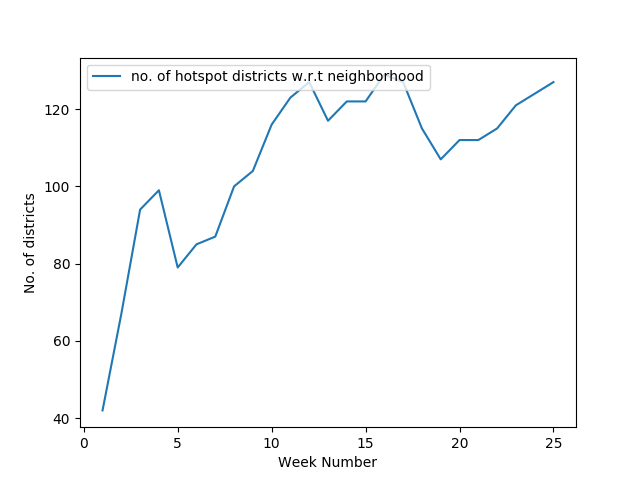
\includegraphics[scale=0.8]{analysis1.png}\\\\

}

\end{enumerate}

\end{document}


